\documentclass[14pt, a4paper]{report} % или article, если не нужен увеличенный базовый шрифт
\usepackage[utf8]{inputenc}
\usepackage[T2A]{fontenc}
\usepackage[russian]{babel}
\usepackage{array}
\usepackage{graphicx}
\usepackage{ulem}
\usepackage{geometry}
\geometry{top=2cm, bottom=2cm, left=2cm, right=2cm}
\usepackage{tabularx}
\usepackage{amsmath}
\usepackage{amssymb}
\usepackage{multirow}
\usepackage{booktabs}
\usepackage{float}
\usepackage{tabularx}
\usepackage{booktabs}
\usepackage{siunitx}
\usepackage{indentfirst}
\usepackage{placeins}
\usepackage{lipsum}
\usepackage{longtable}
\usepackage{csquotes}
\usepackage[style=gost-numeric,sorting=none]{biblatex}
\usepackage{enumitem}
\usepackage{caption}

\captionsetup[table]{position=top, singlelinecheck=false, justification=raggedleft}



\addbibresource{references.bib}
\usepackage{titlesec}
\titleformat{\chapter}[display]
    {\normalfont\huge\bfseries}
    {\chaptertitlename\ \thechapter}
    {20pt}
    {\Huge}
\usepackage{booktabs}
\usepackage{makecell}
\graphicspath{{Image/}}

\geometry{
    a4paper,
    total={170mm,257mm},
    left=20mm,
    top=20mm,
}

\newcommand{\specialcell}[2][c]{%
    \begin{tabular}[#1]{@{}c@{}}#2\end{tabular}%
}

\usepackage{etoolbox}
\patchcmd{\thebibliography}
  {\chapter*{\bibname}}
  {\section*{\centering СПИСОК ЛИТЕРАТУРЫ}}
  {}{}
\patchcmd{\thebibliography}
  {\addcontentsline{toc}{chapter}{\bibname}}
  {\addcontentsline{toc}{section}{СПИСОК ЛИТЕРАТУРЫ}}
  {}{}


\usepackage{setspace}
\onehalfspacing


% Для подчеркивания текста, аналогичного .underline в Word
\newcommand{\und}[1]{\uline{#1}}

\begin{document}

% Титульный лист
\begin{titlepage}
    \centering
    \noindent
    \begin{tabular}{@{}p{0.25\textwidth} p{0.7\textwidth}@{}}
        \raisebox{-\totalheight}{
\includegraphics[width=0.8in, height=0.9in]{imgs/BMSTU.jpg}} &
        \textbf{Министерство науки и высшего образования Российской Федерации} \\
        & \\
        & \textbf{Федеральное государственное бюджетное образовательное} \\
        & \textbf{учреждение} \\
        & \\
        & \textbf{высшего образования} \\
        & \\
        & \textbf{«Московский государственный технический университет} \\
        & \\
        & \textbf{имени Н.Э. Баумана} \\
        & \\
        & \textbf{(национальный исследовательский университет)»} \\
        & \\
        & \textbf{(МГТУ им. Н.Э. Баумана)} \\
    \end{tabular}

    \vspace{1cm}
    ФАКУЛЬТЕТ \und{«СПЕЦИАЛЬНОЕ МАШИНОСТРОЕНИЕ»}

    \vspace{0.5cm}
    КАФЕДРА \und{«РАКЕТНЫЕ И ИМПУЛЬСНЫЕ СИСТЕМЫ» (СМ-6)}

    \vspace{2cm}
    \textbf{РАСЧЕТНО-ПОЯСНИТЕЛЬНАЯ ЗАПИСКА}

    \vspace{1cm}
    \textbf{\textit{К КУРСОВОЙ РАБОТЕ}}

    \vspace{1cm}
    \textbf{\textit{НА ТЕМУ:}}

    \vspace{0.5cm}
    \textbf{\textit{\und{«Баллистическое проектирование артиллерийских орудий»}}}

    \vspace{1.5cm}
    \textbf{Вариант 24}

    \vspace{2cm}
    \begin{flushleft}
        Студент \und{СМ6-72} \hfill \underline{\hspace{5cm}} \hfill \und{М.В. Ерофеев} \\
        \hspace{4.8cm} (Группа) \hspace{2.3cm} (Подпись, дата) \hspace{1.8cm} (И.О.Фамилия) \\[1cm]
        Руководитель курсовой работы \hfill \underline{\hspace{5cm}} \hfill \und{В.А. Федулов} \\
        \hspace{7.5cm} (Подпись, дата) \hspace{1.8cm} (И.О.Фамилия)
    \end{flushleft}

    \vfill
    \centering
    \textit{2025 г.}

    \newpage % Начало второй страницы (Задание)

    \centering
    \textbf{Министерство науки и высшего образования Российской Федерации}

    \textbf{Федеральное государственное бюджетное образовательное учреждение}

    \textbf{высшего образования}

    \textbf{«Московский государственный технический университет имени Н.Э. Баумана}

    \textbf{(национальный исследовательский университет)»}

    \textbf{(МГТУ им. Н.Э. Баумана)}

    \vspace{1cm}
    УТВЕРЖДАЮ

    \vspace{0.5cm}
    Заведующий кафедрой \und{СМ6} \\
    \hspace{1.5cm} (Индекс) \\[0.5cm]
    \underline{\hspace{5cm}} \und{В.М.Кашин} \\
    \hspace{0.5cm} (И.О.Фамилия) \\[0.5cm]
    « \underline{\hspace{1cm}} » \underline{\hspace{3cm}} 20 \underline{\hspace{1cm}} г.

    \vspace{2cm}
    \textbf{ЗАДАНИЕ}

    \textbf{на выполнение курсовой работы}

    \vspace{1cm}
    \begin{flushleft}
        по дисциплине \und{Газовая динамика} \hfill \underline{\hspace{7cm}} \\[0.5cm]
        Студент группы \und{СМ6-72} \\[0.5cm]
        \underline{\hspace{12cm}} \und{Ерофеев Максим Викторович} \\
        \hspace{5cm} (Фамилия, имя, отчество) \\[0.5cm]
        Тема курсовой работы \und{Баллистическое проектирование артиллерийских орудий} \\
        \und{на сжатом газе} \\[0.5cm]
        Направленность КР (учебная, исследовательская, практическая, производственная, др.) \\
        \und{Учебная} \hfill \underline{\hspace{7cm}} \\[0.5cm]
        Источник тематики (кафедра, предприятие, НИР) \und{Кафедра} \hfill \underline{\hspace{5cm}} \\[0.5cm]
        График выполнения работы: 25\% к \und{4} нед., 50\% к \und{8} нед., 75\% к \und{12} нед., 100\% к \und{14} нед. \\[1cm]
        \textbf{\textit{Задание}} \und{Найти оптимальные параметры ствола и условий заряжания при решении обратной задачи внутренней баллистики. При этом $d = 85$ мм, $q =$ 5 кг, $ v_{\text{pm}} = 950 $ м/с, тип орудия – НР, тип математической модели – квазиодномерная (КМ), критерий оптимальности – $Z_{\text{B1}}$, $p^{\text{max}}_{\text{m}}$ = 390 МПа, $l^{\text{max}}_{\text{m}}$ = 65 ед.d, $v_{\text{pm-50}}$ = 850 м/с, $p_{\text{mz+5}}0 = $ 180 МПа.} \\[1cm]
        \textbf{\textit{Оформление курсовой работы:}} \\[0.5cm]
        Расчетно-пояснительная записка на \underline{\hspace{2cm}} листах формата А4. \\[0.5cm]
        \underline{\hspace{15cm}} \\
        \underline{\hspace{15cm}} \\
        \underline{\hspace{15cm}} \\
        \underline{\hspace{15cm}} \\[1.5cm]
        Дата выдачи задания «\und{13}» \und{сентября} \und{2024} г. \\[2cm]
        \textbf{Руководитель курсовой работы} \hfill \underline{\hspace{5cm}} \hfill \und{В.А. Федулов} \\
        \hspace{8cm} (Подпись, дата) \hspace{2cm} (И.О.Фамилия) \\[1.5cm]
        \textbf{Студент} \hfill \underline{\hspace{5cm}} \hfill \und{М.В. Ерофеев} \\
        \hspace{8cm} (Подпись, дата) \hspace{2cm} (И.О.Фамилия)
    \end{flushleft}

\end{titlepage}


\tableofcontents

\newpage
\section*{Введение}
Данная курсовая работа посвящена нахождению оптимальных параметров артиллерийского орудия и условий заряжания путем решения обратной задачи внутреннй баллистики.
Ключевым критерием оптимальности решения является критерий качества баллистического решения $Z_{\text{B1}}$. 

Решение должно удовлетворять следующим требованиям: 
\begin{itemize}
    \item  $p_{\text{m}}^{\text{max}}$ $\leq$ 390 МПа
    \item $l_{\text{m}}^{\text{max}}$ $\leq$ 65 ед.d
\end{itemize}

Также на решение наложены следующие ограничения: 
\begin{itemize}
    \item  $v_{\text{pm-50}}$ = 830 $\text{м/c}$
    \item $p_{\text{mz+50}}$ = 180 МПа
\end{itemize}

Условие задания: 
\begin{itemize}
    \item $d$ = 85 мм
    \item $q$ = 5 кг
    \item $v_{\text{pm}}$ = 950 $\text{м/c}$
    \item Тип орудения -- нарезное (НР)
    \item Тип мат. модели -- квазиодномерная (КМ)
\end{itemize}

Данная задача будет решаться с использованием мат. аппарата квазиодномерной модели внутренней.
баллистики. Также использованы методы оптимизации для нахождения оптимального решения обратной задачи с учетом критериев и ограничений.

Вычисления проводились с помощью языка программирования Python с использованием библиотеки PyBallistics [1], визуализация данных осуществлялась 
через библиотеку Matplotlib [2].

\newpage
\chapter{Прямая задача внутренней баллистики}
\section{Описание математической модели}

Выстрел предствавляет собой довольно сложный быстропротекающий физико-химический процесс. Его физическая сущность состоит в том, что при сгорании порохового заряда образуются газообразные продукты сгорания под большим давлением, 
под действием которого снаряд выталкивается из канала ствола с огромной скоростью. Прямая задача состоит в том, чтобы описать движение снаряда массой $q$ по каналу ствола диаметра $d$ под действием давления продуктов сгорания заряда пороха массой $\omega$, находящимся в объеме $W_0$. Схема процесса вместе с качественными распределениями давления и скорости представлена на рисунке 1.
Для упрощения вводится ствол с камерой приведенной длины $l_0$, имеющей тот же обеъем $W_0$, но с диаметром, равным калибру ствола $d$. Схема упрощения представлена на рисунке 1.2. 

\begin{figure}[h!]
\centering

\includegraphics[width=0.45\textheight]{imgs/1.jpg}
\caption{Схема процесса выстрела}
\end{figure}

\begin{figure}[h]
\centering
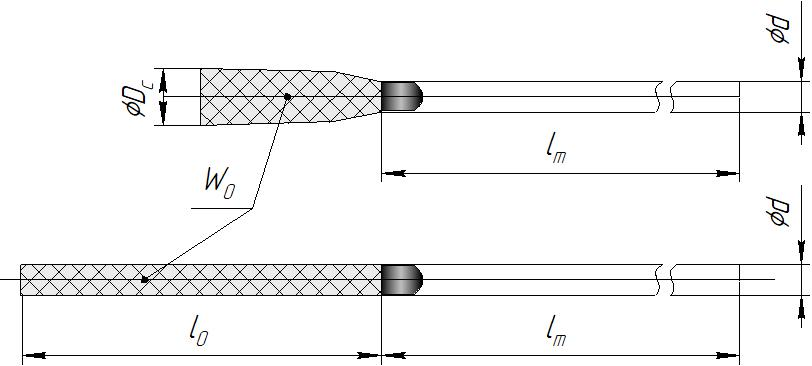
\includegraphics[width=0.5\textheight]{imgs/2.jpg}
\caption{Схема упрощения}
\end{figure}

Наиболее соверменным и точным описанием процесса выстрела является газодинамический подход, 
по размерности в нашем случае модель является одномерной (квазиодномерной). Эта модель выстрела содержит некоторые допущения: 
\begin{itemize}
    \item Гипотеза односкоростной газопороховой смеси (ОГПС)
    \item Геометрический закон горения пороха
\end{itemize}


    В пространстве между дном ствола и дном снаряда (заснарядный объём) в процессе движения снаряда 
по каналу ствола находятся газообразные продукты сгорания пороха и конденсированные частицы несгоревшего пороха.
Для упрощения принимается, что пороховые газы и конденсированные элементы представляют собой гомогенную смесь, которая движется 
с общей скоростью. Такое допущение называется гипотезой односкоростной газопороховой смеси (ОГПС). Уравнение состояния ОГПС представляется в виде: 

\begin{equation}
\varepsilon = \frac{p}{k - 1} \left( \frac{1}{\rho} - \frac{1 - \psi}{\delta} - b \psi \right) + (1 - \psi) \frac{f}{k - 1},
\label{eq:epsilon}
\end{equation}
где $\varepsilon$ -- удельная внутрення энергия ОГПС, $\rho$ -- плотность ОГПС, $b$ -- коволюм порохового газа (эффективный собственный объём молекул), $k$ -- показатель адиабаты, 
$\psi$ = $\omega_b$ / $\omega$ -- отношение массы сгоревшего элемента у его исходной массе, $\omega_b$ -- масса сгоревшего пороха, $\omega$ -- исходная масса пороха. $\delta$ -- плотность пороха. 

Геометрический закон горения пороха выражается в виде формулы (1): 

\begin{equation}
\frac{dz}{dt} = \frac{p^\nu}{I_e}, 
\label{eq:1}
\end{equation}
где  $p$ -- давление газа, $\nu$ -- показатель степени
в законе горения. В артиллерии, как правило, $\nu$ = 1. $z$ = $e$ /$e_1$ -- безразмерная толщина сгоревшего свода порохового элемента. В свою очередь
$e$ -- координата текущего положения поверхности горения, а $e_1$ -- полная толщина горящего свода порохового элемента. $I_e$ -- полный импульс давления пороховых газов:
\[
I_e = \int_0^{t_e} p^v  dt = \frac{e_1}{u_1},
\]

где $u_1$ -- скорость горения при единичном горении, определяемая экспериментальным путем.

Далее рассмотрим систему уравнений для газодинамической задачи в приближении ОГПС. ОГПС в данном случае представляет собой «псевдогаз», её движение в заснарядном
объёме описывается стандартными уравнениями сохранения массы, импульса и энергии в лагранжевых координатах: 

\begin{equation}
\frac{\partial v}{\partial m} = \frac{d}{dt}\left(\frac{1}{\rho S}\right)
\end{equation}

\begin{equation}
\frac{dv}{dt} + S\frac{\partial p}{\partial m} = 0,
\end{equation}

\begin{equation}
\frac{d\epsilon}{dt} + p\frac{\partial}{\partial m}(vS) = 0.
\end{equation}

Здесь $m$ -- массовая лагранжева координата.

Для математического описания процесса выстрела необходимо установить закономерность газообразования, то есть связь между геометрическими размерами порохового элемента (ПЭ) и количеством пороховых газов (ПГ), образованных в процессе выгорания заряда, а также интенсивностью их образования. Такую зависимость называют функцией газоприхода $\psi(z)$:

\begin{equation}
\psi(z) = \kappa z (1 + \lambda z + \mu z^2),
\end{equation}

где $k, \lambda, \mu$ -- коэффиценты формы порохового зерна (порохового элемента).
На практике для расчётов пользуются упрощенной формой записи данного закона:

\begin{equation}
\psi(z) = \kappa z (1 + \lambda z),
\end{equation}
где коэффицинты $k, \lambda$ определяются путём приравнивания функций $\psi$, полученных расчётом по формулам (1.6) и (1.7) в точках $z$ = 0.5 и $z$ = 1.

Чтобы замкнуть систему уравнений, необходимо записать уравнение движения снаряда по каналу ствола:

\begin{equation}
q \, \frac{d v_{p}}{d t} = S p_{p} - R,
\end{equation}
где $q$-- масса снаряда, $v_p$ -- скорость скорость снаряда, $S$-- площадь поперечного сечения канала ствола, $ p_{p}$ -- давление на дно снаряда, $R$ -- суммарная сила сопротивлению движения снаряда. 

Запишем теперь полученную систему уравнений: 

\[
\left\{
\begin{array}{l}
\dfrac{\partial v}{\partial m} = \dfrac{d}{dt}\left(\dfrac{1}{\rho S}\right) \\[1.5ex]
\dfrac{dv}{dt} + S\dfrac{\partial p}{\partial m} = 0 \\[1.5ex]
\dfrac{d\varepsilon}{dt} + p\dfrac{\partial}{\partial m}(vS) = 0 \\[1.5ex]
\varepsilon = \dfrac{p}{k - 1} \left( \dfrac{1}{\rho} - \dfrac{1 - \psi}{\delta} - b \psi \right) + (1 - \psi) \dfrac{f}{k - 1} \\[1.5ex]
\dfrac{dz}{dt} = \dfrac{p^\nu}{I_e} \\[1.5ex]
q \, \dfrac{d v_{p}}{d t} = S p_{p} - R
\end{array}
\right.
\]

В дальнейшем данная система уравнений будет преобразовываться, так что это не конечный вид.

\section{Сила сопротивления движению снаряда по каналу ствола}

В процессе выстрела на снаряд действует не только сила давления пороховых газов, но и сила врезания ведущих поясков снаряда в нарезы, сила трения ведущих устройств о поверхность нарезов и сила сопротивления сжатию столба воздуха перед снарядом. 

Начальный этап движения снаряда включает в себя врезание ведущих поисков в нарезы. Это весьма сложный процесс, в котором необходимо учитывать пластичекую деформацию медного пояска снаряда. В расчетах применяется гипотеза мнгновенного врезания: движения снаряда начинается тогда, когда давление на дно снаряда достигает 
некоторого условного предела, называемого давлением форсирования $p_0$. Для разных типов орудий значение данного предела может отличаться. Так, для нарезных стволов и снарядов с одним ведущим поясков $p_0$ = 30 МПа, что соответсвует данному варианту курсовой работы.

Классическим решением учета большей части форм сопротивления является домножение массы снаряда на некоторый коэффициент фиктивности $\phi$.

Рассмотрим две наибольшие состовляющие сил сопротивления движению снаряда -- сила, возникающая при сжатии столба воздуха во время движения снаряда и сила сопротивления движения по нарезам. Тогда суммарная сила сопротивления
движению снаряда представляет: 

\begin{equation}
R = p_a S + R_b,
\end{equation}
где $p_a$ -- давление воздушного столба перед снарядом, $R_b$ -- сила взаимодействия ведущих устройств (нарезов)
со снарядом.

Противодействие воздуха перед снарядом имеет сущесвтенное влияние, которое необходимо учитывать. Особенно это проявляется при движении снаряда 
со сверхзвуковой скоростью относительно невозмущенного воздуха. Данный фактор можно приближеннго учесть с помощью известной зависимости для точного решения задачи о поршне, сжимающем газ:

\begin{equation}
P_a = P_{0a} \left(1 + \frac{k_a(k_a+1)}{4} \left(\frac{\upsilon_p}{c_{0a}}\right)^2 + 
k_a \frac{\upsilon_p}{c_{0a}} \sqrt{1 + \left(\frac{k_a+1}{4} \frac{\upsilon_p}{c_{0a}}\right)^2} \right),
\end{equation}
где $k_a$, $P_{0a}$ и $c_{0a}$ — показатель адиабаты, давление и скорость звука в невозмущённом воздухе.

Для учёта силы трения в нарезах используется данная формула коэффициента фиктивной массы снаряда: 

\begin{equation}
\varphi = \varphi_1 + \frac{\omega}{3q}.
\label{eq:phi_equation}
\end{equation}
где $\varphi_1 \approx$  1.02.

\section{Учёт потерь на теплоотдачу в стенки ствола}

Основым источником теплопотерь при выстреле является теплоотдача в стенки ствола. Интенсивность этого процесса определяется разностью температур раскалённых пороховых газов и холодной стенки ствола. Ниже представлен упрощённый расчёт, который применим и к газодинамической модели.
Рассмотрим основное уравнение внутренней баллистики с учётом тепловых потерь:

\begin{equation}
\frac{k-1}{2} \varphi q v_p^2 = f \omega \psi - p_m \left( W_p - \frac{\omega}{\delta} + \left( \frac{1}{\delta} - b \right) \omega \psi \right) + p_{\text{ign}} \left( W_0 - \frac{\omega}{\delta} \right) - Q_w.
\end{equation}

В свою очередь, затраченная на теплоотдачу энергия может быть вычислена из следующих соображений:

\begin{equation}
\frac{dQ_{w}}{dt} = S_{w} q_{w},
\end{equation}

\begin{equation}
q_{w} = \mathrm{Nu} \frac{\lambda_g}{d} (T - T_{w}) = 0.023 \, \mathrm{Re}^{0.8} \, \mathrm{Pr}^{0.4} \frac{\lambda_g}{d} (T - T_{w}),
\end{equation}
где Nu -- число Нуссельта; Re -- число Рейнольдса; Pr -- число Прандтля (для порохового газа Pr = 0.74); $\lambda_g$ -- теплопроводность пороховых газов; $d$ -- диаметр канала (калибр); $S_w$ -- площадь поверхности теплоотдачи (площадь контакта пороховых газов со стволом).

Число Рейнольдса определяется по формуле:

\begin{equation}
\mathrm{Re} = \frac{\rho v d}{\mu},
\end{equation}
где $v$ -- средняя скорость потока; $\mu$ -- коэффициент динамической вязкости.
 
Средняя температура стенки \( T_w \) определяется по приближенной методике Р. Е. Соркина:

\begin{equation}
\frac{d\eta_T}{dt} = \frac{2 \mathrm{Nu}^2 \lambda_g^2}{d^2 c_b \rho_b \lambda_b} \left( T - T_0 - \sqrt{n_T} \right),
\end{equation}
где \( \sqrt{n_T} = T_w - T_0 \); \( n_T(0) = 0 \); \( c_b, \, \rho_b \) и \( \lambda_b \) — теплоёмкость, плотность и теплопроводность материала ствола соответственно; \( T_0 \) — начальная температура.

Коэффициент динамической вязкости пороховых газов может быть аппроксимирован формулой Сазерленда:

\begin{equation}
\mu = \mu_0 \mathrm{Pr} \frac{T_{cs} + T_{0s}}{T_{cs} + T} \left( \frac{T}{T_{0s}} \right)^{1.5},
\tag{1.43}
\end{equation}

где \( \mu_0 = 0.175 \cdot 10^{-4} \, \text{Па·с} \); \( T_{0s} = 273 \, \text{K} \); \( T_{cs} = 628 \, \text{K} \).

Площадь контакта \( S_w \) пороховых газов со стволом увеличивается по мере движения снаряда, причём увеличивается за счёт новой, «холодной» площади канала ствола. Вследствие этого средняя температура стенки \( T_w \) уменьшается.

Это можно учесть добавлением слагаемого \( v_n \) в формуле (1.42):

\begin{equation}
\frac{dn_T}{dt} = \frac{2 \mathrm{Nu}^2 \lambda_g^2}{d^2 c_b \rho_b \lambda_b} \left( T - T_0 - \sqrt{n_T} \right) + v_n.
\end{equation}

Выражение для \( v_\eta \) можно получить из следующих соображений: пусть в определённый момент времени средняя температура поверхности ствола за снарядом составляет \( T_w \). Снаряд движется со скоростью \( v_p \) и за время \( dt \) к площади теплоотдачи добавляется новая поверхность ствола с температурой \( T_{w0} \). При этом средняя температура ствола за время \( dt \) будет равна:

Отсюда можно определить \( v_n \):

\[
v_n = \lim_{dt \to 0} \frac{\eta_{T1} - \eta_T}{dt} = \lim_{dt \to 0} \frac{(T_{w1} - T_{w0})^2 - (T_w - T_{w0})^2}{dt} = -\frac{2v_p (T_w - T_{w0})^2}{x_p} = -\frac{2v_p \eta_T}{x_p}.
\]

Учёт теплоотдачи в стенки ствола в газодинамических моделях внутренней баллистики должен осуществляться совместно с решением пространственной задачи нагрева ствола. В большинстве случаев такая задача сопоставима по трудоёмкости с решением задачи внутренней
баллистики. При этом следует отметить, что в случае единичного выстрела учёт нагрева стенок ствола слабо влияет на основные баллистические характеристики. Поэтому, в ряде случаев можно считать температуру стенок ствола постоянной на протяжении выстрела [3].

Стоит отметить, что в случае квазиодномерной постановки расчёт теплоотдачи необходимо применть к каждой ячейке на расчётной сетке.

\section{Особенности расчёта смеси порохов}

Рассмотрим случай, когда пороховой заряд состоит из смеси порохов, которые могут характеризоватсья различными параметрами и формой порохового элемента. В данном случае продукты сгорания различных марок порохов образуют общую смесь газов.

Уравнение состояние ОГПС принимает следующий вид:

\begin{equation}
\varepsilon = \frac{1}{k-1} P_m \left[ \frac{1}{\rho} - \sum_{i=1}^N \frac{C_i (1 - \psi_i)}{\delta_i} - \sum_{i=1}^N C_i \psi_i b_i \right] + \sum_{i=1}^N C_i (1 - \psi_i) \frac{f_i}{k_i - 1}; 
\end{equation}

\begin{equation}
k = 1 + \frac{\sum_{i=1}^N C_i \psi_i R_{g,i}}{\sum_{i=1}^N \dfrac{C_i \psi_i R_{g,i}}{k_i - 1}}; \quad C_i = \frac{\omega_i}{\sum_{j=1}^N \omega_j},
\end{equation}
где \( C_i, \psi_i, \delta_i, b_i, f_i, k_i, R_{g,i}, \omega_i \) -- массовая доля пороховых газов, доля сгоревшего пороха, плотность пороха, коволюм порохового газа, сила пороха, показатель адиабаты, газовая постоянная пороховых газов и масса \(i\)-й навески смеси соответственно.
\newpage
\begin{thebibliography}{9}
\bibitem{} \textbf{PyBallistics}
\bibitem{} \textbf{Matplotlib} 
\bibitem{} \textbf{Основная метода} 

\end{thebibliography}

\end{document}